\documentclass[11pt,a4paper]{article}

\usepackage[margin=1in]{geometry}
\usepackage{amsmath,amssymb,amsthm}
\usepackage{booktabs}
\usepackage{tikz}
\usetikzlibrary{arrows.meta,positioning}
\usepackage[round]{natbib}
\usepackage[colorlinks=true,linkcolor=black,citecolor=black,urlcolor=blue]{hyperref}
\usepackage{parskip}
\usepackage{caption}

\newtheorem{proposition}{Proposition}
\newcommand{\E}{\mathbb{E}}
\setlength{\emergencystretch}{1.5em}

\title{\textbf{A Multi-Timeframe ARX Direction Model on Five-Minute Bars}\\[0.4em]
\large Design, Walk-Forward Evidence, and What the Signal Really Is}
\author{Khanh Nguyen}
\date{}

\begin{document}
\maketitle

\begin{abstract}
\noindent We design and test an intraday direction model for 431 S\&P~500 stocks on 5-minute
bars. An ARX regression forecasts the next bar's return from five lags of returns and of a bounded
flow-pressure proxy built from each bar. Forecasts from six timeframes, 5 minutes to 4 hours, are put
on a common scale and averaged, and the book goes long or short on the sign of the average. Every
design choice is explained, the walk-forward is checked for look-ahead with a test that is shown to
catch a deliberate leak, and results are reported on returns a trade can earn. Four findings. First,
using the midpoint of the bar's range instead of the close raises the hit rate from $0.506$ to
$0.689$, but only on the midpoint itself; on tradable returns the midpoint model is right
$49.0\%$ of the time. Second, the close model has a small, very steady gross edge: hit rate
$0.506$, gross Sharpe $4.99$ when trades are filled at the next bar's open. Third, the edge is a
one-bar reversal; the flow proxy adds nothing. Fourth, combining timeframes keeps half the edge at a
third of the trading, and a confidence filter cuts trading by $93\%$; the results are robust to
the number of lags, the training window and the filter level. Whether the edge survives trading costs
is summarised in Section~\ref{sec:discussion} and treated fully in a companion paper.
\end{abstract}

%=====================================================================
\section{Introduction}
\label{sec:intro}

\paragraph{Motivation.} Short-horizon stock returns are not pure noise. Returns reverse over days and
weeks \citep{lehmann1990,jegadeesh1995}; within the day, the first half hour predicts the last
\citep{gao2018}, and returns at the same time of day are correlated across days \citep{heston2010}. At
the shortest horizons, order flow carries information that prices absorb over several trades
\citep{kyle1985,hasbrouck1991}. These effects operate at different horizons, from minutes to hours. A
model that looks at one horizon only sees one of them.

\paragraph{The idea.} Forecast the next bar's return at several horizons with the same simple model, put
the forecasts on a common scale, and average them. If the horizons capture different effects, their
forecasts should be weakly correlated, and the average should keep most of the predictive content while
changing position less often. Trading less matters because every change of position costs money.

\paragraph{Why OHLCV bars.} Trade-and-quote data with signed trades is expensive and heavy; 5-minute bars
exist for every liquid asset. The model therefore uses a flow proxy built from the bar itself. A
companion paper shows that some regressions on bar data measure arithmetic rather than information, so
here every result is scored on returns that a trade can actually earn.

\paragraph{Contributions.}
\begin{enumerate}
\item A complete, reproducible design, with the reason for every choice (Section~\ref{sec:model}).
\item A walk-forward protocol whose look-ahead test is itself tested with a deliberate leak
(Section~\ref{sec:protocol}).
\item Evidence on what the signal is: its hit rate, where its profit comes from, why a hit rate near one
half can give a high Sharpe ratio, and which coefficients carry it (Section~\ref{sec:results}).
\item Evidence that combining horizons works through turnover, and that this is robust to the main
parameters (Sections~\ref{sec:mtf}--\ref{sec:sens}).
\end{enumerate}

%=====================================================================
\section{The model}
\label{sec:model}

Every input at time $t$ is known at the end of bar $t$. Each step below states what is done and why.

\paragraph{Step 1: returns.} $r_t = 10^4(\log p_t - \log p_{t-1})$, in basis points (bps), so that stocks
with different prices can be pooled. Two prices are compared. CLOSE uses $p_t=C_t$. MID uses the midpoint
of the bar's range, $p_t=(H_t+L_t)/2$, a common choice because it looks like a quote midpoint and is less
noisy than the close. It is not a quote midpoint: it is an average over the bar, known only after the bar
ends, and no order can be filled at it. Section~\ref{sec:mid} shows why this matters.

\paragraph{Step 2: flow-pressure proxy.}
\begin{equation}
x_t = \tanh\!\Big(\underbrace{\operatorname{sign}(C_t-O_t)}_{\text{direction}}\cdot
\underbrace{\frac{|C_t-O_t|}{H_t-L_t}}_{\text{dominance}}\cdot\underbrace{\log(1+V_t)}_{\text{activity}}\Big).
\label{eq:x}
\end{equation}
The direction says which side won the bar, the standard bar-level substitute for a trade sign. The
body-to-range ratio says how decisively: a bar that opens at its low and closes at its high scores one,
a bar that ends where it began scores zero. The log of volume gives busy bars more weight but grows slowly,
so a volume spike does not dominate. The $\tanh$ keeps $x_t$ in $(-1,1)$, so one extreme bar cannot
dominate a least-squares fit. The plain sign $\operatorname{sign}(C_t-O_t)$ is kept as a comparison.

\paragraph{Step 3: ARX forecast.}
\begin{equation}
\hat r_{t+1} = \beta_0 + \sum_{k=1}^{L}\beta_k\, r_{t+1-k} + \sum_{k=1}^{L}\gamma_k\, x_{t+1-k},\qquad L=5.
\label{eq:arx}
\end{equation}
The return lags capture momentum ($\beta_1>0$) or reversal ($\beta_1<0$); the flow lags capture price
impact that arrives after the bar. The model is linear because the effects are small and noisy, and a
linear model has few parameters and a closed-form fit that can be re-estimated thousands of times.
This is also the forecasting form of the \citet{hasbrouck1991} VAR: substituting the VAR's flow
equation into its price equation gives a forecast linear in exactly these regressors. $L=5$ covers 25
minutes at the 5-minute timeframe; Section~\ref{sec:sens} shows that 1, 3 or 10 lags give the same
results.

\paragraph{Step 4: score.}
\begin{equation}
s_t = \tanh(\hat r_{t+1}/\sigma_t),
\label{eq:score}
\end{equation}
where $\sigma_t$ is the standard deviation of that timeframe's returns over the last 20
sessions. A forecast of 2 bps means much more for a quiet stock at 5 minutes than for a volatile stock at
4 hours; dividing by $\sigma_t$ puts forecasts on one scale before they are averaged. The $\tanh$ bounds
the score. For a single timeframe the score has the same sign as the forecast, since $\sigma_t>0$ and
$\tanh$ is increasing with $\tanh(0)=0$, so trading the score and trading the forecast give the same
positions. In practice the average $|s_t|$ is $0.033$--$0.135$ across timeframes and the average
$|S_t|$ is $0.036$, where $\tanh(z)\approx z$.

\paragraph{Step 5: combine timeframes.} Steps 1--4 run on bars of 5m, 15m, 30m, 1h, 2h and 4h, built from
the 5-minute bars within each session. These cover the horizons of the effects in the introduction:
5--15 minutes for order flow and bounce, 30--60 minutes for intraday trend and reversal, 2--4 hours for
the state of the day. At each 5-minute bar a timeframe contributes the score of its last \emph{finished}
bar, so no partly formed bar is used. The combined score is
\begin{equation}
S_t = \frac{\sum_\tau w_\tau\, s^{(\tau)}_t}{\sum_\tau |w_\tau|}.
\label{eq:mtf}
\end{equation}
Two weightings are fixed before testing: equal weights, and weights learned on 2021 only (each
timeframe's gross profit per unit of trading in 2021, floored at zero) and then frozen.

\paragraph{Step 6: position.} Long one unit if $S_t>0$, short one unit if $S_t<0$. Two versions trade less:
\emph{size by score}, $w_t=S_t$, and a \emph{confidence filter},
\[
w_t=\begin{cases}\operatorname{sign}(S_t) & \text{if } |S_t|\ge q,\\ w_{t-1} & \text{otherwise,}\end{cases}
\]
where $q$ is the 75th percentile of $|S|$ over the previous 2{,}000 bars. A weak score keeps
the current position, so no trade happens. The level 0.75 was fixed before any run; other levels are
in Section~\ref{sec:sens}.

%=====================================================================
\section{Walk-forward protocol and look-ahead tests}
\label{sec:protocol}

\paragraph{Data.} 431 S\&P~500 stocks with 5-minute regular-hours bars from Interactive Brokers for
the whole period, 2019-12-09 to 2025-01-10.

\paragraph{Sessions and the overnight gap.} Timeframe bars are built within each session from 09:30.
The first return of a session is measured from that session's open, so the overnight gap never enters a
series. No target and no position spans two sessions; positions are closed at the end of each session.

\paragraph{Rolling estimation.} Each model is fitted on the last 256 sessions (about one year)
and refitted every 25.6 sessions (about one month). One year is long enough for stable
estimates of eleven coefficients and short enough to follow slow changes; monthly refits keep the model
current without refitting on every bar. A 5-minute model therefore uses about 20{,}000 bars and is refitted
every 2{,}000. Figure~\ref{fig:wf} shows the timing.

\begin{figure}[htbp]
\centering
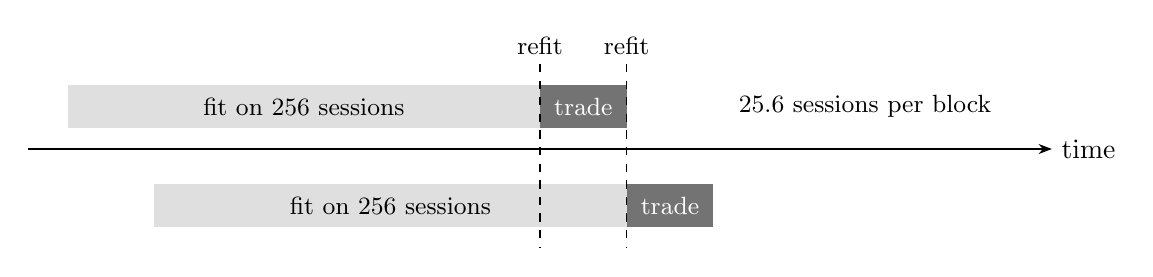
\begin{tikzpicture}[x=1cm,y=0.9cm,>=Stealth]
\draw[->] (0,0) -- (13,0) node[right]{time};
\fill[gray!25] (0.5,0.3) rectangle (6.5,0.9); \node at (3.5,0.6) {\small fit on 256 sessions};
\fill[black!55] (6.5,0.3) rectangle (7.6,0.9); \node[white] at (7.05,0.6) {\small trade};
\fill[gray!25] (1.6,-0.5) rectangle (7.6,-1.1); \node at (4.6,-0.8) {\small fit on 256 sessions};
\fill[black!55] (7.6,-0.5) rectangle (8.7,-1.1); \node[white] at (8.15,-0.8) {\small trade};
\draw[dashed] (6.5,1.2) -- (6.5,-1.4); \node[above] at (6.5,1.2) {\small refit};
\draw[dashed] (7.6,1.2) -- (7.6,-1.4); \node[above] at (7.6,1.2) {\small refit};
\node[right] at (8.9,0.6) {\small 25.6 sessions per block};
\end{tikzpicture}
\caption{Rolling walk-forward. A model fitted on the previous 256 sessions trades the next 25.6
sessions, then is refitted. Every training target is known before the first trade it is used for.}
\label{fig:wf}
\end{figure}

\paragraph{Evaluation period.} All strategies are scored on the same 78{,}205 five-minute bars, 2020-12-18 to
2025-01-10, as an equal-weight book of 426.6 stocks on average. Learned weights use data before 2022
only, so January 2022 -- January 2025 is a hold-out.

\paragraph{Fill.} A decision at the end of bar $t$ is filled at the open of bar $t+1$, the first print
after the signal, which is what a market order sent at the bar close receives. Results with a fill at the
close of bar $t$, a common but optimistic backtest convention, are shown for comparison.

\paragraph{Look-ahead tests.} A walk-forward can still leak future data through a feature, a scaling
statistic or the refit schedule. We test this directly. The whole pipeline is run twice, on the full data
and on data cut at bar $T$; every score, position and cost at or before $T$ must be identical, because
nothing computed at time $t$ may depend on later data. Cuts are placed at 13:25, where every timeframe's
bar is complete, and at the session end, for 3 stocks and 3 dates: 18 of
18 runs are identical. A test that never fails proves nothing, so we also ran it after deliberately
leaking the next bar into the proxy: it fails, as it should. The first version of the test cut data
only at session ends, where no decision is made, and missed this leak; cutting mid-session fixed it.

\paragraph{Measures.} \emph{Hit rate}: the share of bars on which the sign of the position matches the sign
of the next return. \emph{Gross return per bar}: the average book return in bps before costs.
\emph{Turnover}: the average of $|w_t-w_{t-1}|$ per bar; a switch from long to short counts two.
\emph{Breakeven half-spread}: gross return per bar divided by turnover. It is the largest cost per unit
of position change at which the book still breaks even, and it is the number that decides whether a
strategy can be traded; Sharpe ratio does not. Sharpe ratios are annualised with $78\times252$ bars.

%=====================================================================
\section{Results}
\label{sec:results}

\subsection{MID beats CLOSE only on its own target}
\label{sec:mid}

\begin{table}[htbp]
\centering
\caption{Out-of-sample hit rate on each timeframe's next bar, average over stocks.}
\label{tab:midacc}
\small
\begin{tabular}{@{}lrrrrrr@{}}
\toprule
& 5m & 15m & 30m & 1h & 2h & 4h \\
\midrule
MID, scored on next midpoint return & $0.689$ & $0.704$ & $0.710$ & $0.726$ & $0.748$ & $0.775$ \\
MID, scored on next close return & $0.490$ & $0.497$ & $0.497$ & $0.500$ & $0.502$ & $0.494$ \\
CLOSE, scored on next close return & $0.506$ & $0.502$ & $0.501$ & $0.501$ & $0.502$ & $0.507$ \\
\bottomrule
\end{tabular}
\end{table}

The MID model predicts the next midpoint return correctly $0.689$ of the time at 5 minutes and
$0.775$ at 4 hours, far above anything the close model achieves. On the next close return it is
right $0.490$--$0.502$ of the time at every timeframe, i.e.\ no better than a coin. The reason
is exact: $\log\mathrm{mid}_{t+1}-\log\mathrm{mid}_t = (\log\mathrm{mid}_{t+1}-\log C_t) +
(\log C_t-\log\mathrm{mid}_t)$. The second term is fixed when bar $t$ closes and is positive when the bar
closes in the upper half of its range, which is usually a bar that also went up. A model that uses bar
$t$ is therefore partly ``predicting'' a number it already knows. The close-to-close return does not
contain that term. From here on, all models use the close.

\subsection{The 5-minute model and its variants}
\label{sec:close}

\begin{table}[htbp]
\centering
\caption{5-minute versions. Hit rate against the next midpoint, close-to-close and open-to-close
return; gross return and Sharpe with the next-open fill; breakeven (bps) with close and next-open fill;
share of stocks with gross profit.}
\label{tab:var5}
\footnotesize
\setlength{\tabcolsep}{3pt}
\begin{tabular}{@{}lrrrrrrrr@{}}
\toprule
& \multicolumn{3}{c}{Hit rate vs next} & \multicolumn{2}{c}{Gross, next open} & \multicolumn{2}{c}{B/E (bps)} & \\
\cmidrule(lr){2-4}\cmidrule(lr){5-6}\cmidrule(lr){7-8}
Version & MID & CLOSE & OC & bps/bar & Sharpe & close & open & \% stocks \\
\midrule
MID, target $\Delta$MID & $0.689$ & $0.490$ & $0.493$ & $-0.138$ & $-4.14$ & $-0.243$ & $-0.133$ & $7.0$ \\
CLOSE, target $\Delta$CLOSE & $0.431$ & $0.506$ & $0.504$ & $0.098$ & $4.99$ & $0.190$ & $0.103$ & $82.8$ \\
CLOSE, plain-sign proxy & $0.431$ & $0.506$ & $0.504$ & $0.098$ & $5.02$ & $0.190$ & $0.103$ & $85.2$ \\
CLOSE, target OC & $0.453$ & $0.504$ & $0.503$ & $0.075$ & $4.48$ & $0.126$ & $0.080$ & $81.0$ \\
CLOSE, ridge + decay & $0.436$ & $0.506$ & $0.504$ & $0.096$ & $5.14$ & $0.188$ & $0.103$ & $85.4$ \\
\bottomrule
\end{tabular}
\end{table}

The close model is right $0.506$ of the time, earns $0.098$ bps per bar gross, and makes gross profit
in most stocks. Replacing the $\tanh$ proxy by the plain sign, training on the open-to-close return, or
adding ridge shrinkage with decay weighting changes nothing of substance. That the proxy's magnitude
terms add nothing is itself informative: they are built from the same bar as the sign and carry no
further information about the next bar.

\subsection{What the signal is}
\label{sec:signal}

\begin{table}[htbp]
\centering
\caption{Walk-forward coefficients of the 5-minute close model, averaged over 17{,}240 refits
(431 stocks), and the share of refits in which each is positive.}
\label{tab:coef}
\small
\begin{tabular}{@{}lrr@{}}
\toprule
Regressor & Mean & \% positive \\
\midrule
$\beta_0$ & $0.0043$ & $52.3\%$ \\
$r_t$ & $-0.0219$ & $24.1\%$ \\
$r_{t-1}$ & $-0.0072$ & $36.4\%$ \\
$r_{t-2}$ & $-0.0017$ & $45.6\%$ \\
$r_{t-3}$ & $0.0007$ & $52.8\%$ \\
$r_{t-4}$ & $0.0009$ & $53.3\%$ \\
$x_t$ & $-0.0198$ & $48.2\%$ \\
$x_{t-1}$ & $0.0108$ & $51.2\%$ \\
$x_{t-2}$ & $0.0125$ & $51.8\%$ \\
$x_{t-3}$ & $0.0042$ & $50.7\%$ \\
$x_{t-4}$ & $0.0422$ & $55.9\%$ \\
\bottomrule
\end{tabular}
\end{table}

Only one coefficient has a stable sign: the latest return, negative in $76\%$ of refits. Every
flow coefficient is positive in about half of the refits. The model is a one-bar reversal: it buys after a
down bar and sells after an up bar. At five minutes much of such reversal is bid--ask bounce: a close
printed at the bid is followed by prints nearer the middle of the spread \citep{roll1984}. This is the
first sign that the edge may be hard to capture with market orders.

\subsection{Why a hit rate near one half gives a high Sharpe ratio}
\label{sec:why}

The model trades only the sign of its forecast. Its forecasts are tiny: the average $|s_t|=|\hat r_{t+1}|/\sigma_t$ is $0.033$, i.e.\ forecasts are about
$3\%$ of one standard deviation, and useless as predictions of size. What matters is how often the sign is right and how
large the move is when it is right or wrong. With hit rate $p$ and average absolute next returns
$m_{\text{hit}}$ and $m_{\text{miss}}$,
\[
\E[\text{profit per bar}] = \underbrace{(p-\tfrac12)(m_{\text{hit}}+m_{\text{miss}})}_{\text{hit rate}}
+ \underbrace{\tfrac12(m_{\text{hit}}-m_{\text{miss}})}_{\text{larger wins than losses}}.
\]

\begin{table}[htbp]
\centering
\caption{Hit rate and move size (close-to-close return, bps), pooled over stocks and bars, close fill;
the last two columns are shares of stocks.}
\label{tab:hit}
\small
\begin{tabular}{@{}lrrrrr@{}}
\toprule
Strategy & $p$ & $m_{\text{hit}}$ & $m_{\text{miss}}$ & Hit rate $<0.5$ & $<0.5$ and profit \\
\midrule
CLOSE 5m & $0.5059$ & $12.49$ & $12.41$ & $8.8\%$ & $2.3\%$ \\
CLOSE MTF, equal, sign & $0.5024$ & $12.50$ & $12.40$ & $20.0\%$ & $7.7\%$ \\
CLOSE MTF, equal, filtered & $0.5008$ & $12.43$ & $12.38$ & $38.1\%$ & $12.5\%$ \\
MID MTF, equal, filtered & $0.5012$ & $12.34$ & $12.46$ & $31.1\%$ & $1.4\%$ \\
\bottomrule
\end{tabular}
\end{table}

For the 5-minute model $77\%$ of the edge comes from the hit rate and the rest from larger wins.
When $p$ is very close to one half, move size decides: $13\%$ of stocks in the filtered book
are right less than half the time and still profitable, while the MID filtered book is right
$0.5012$ of the time and loses money. Hit rate alone does not show whether a sign strategy makes
money.

The high Sharpe ratio comes from breadth. The correlation between position and next return, the
information coefficient, is $0.0108$. A single stock's daily profit has a Sharpe ratio of $0.78$.
Daily profits of different stocks have an average correlation of $0.025$, so the 431 stocks act like
$36$ independent bets, and the fundamental law of active management \citep{grinold1989} predicts
a portfolio Sharpe of $0.78$ $\times\sqrt{N_{\text{eff}}}\approx$ $4.70$. The realised daily
Sharpe is $4.76$. Many tiny bets give a high Sharpe ratio even when each bet is nearly a coin flip; they
say nothing about whether each bet covers its cost.

\subsection{Combining timeframes}
\label{sec:mtf}

\begin{table}[htbp]
\centering
\caption{Single timeframes, close model, next-open fill unless marked. B/E in bps; last column: share of
months with gross profit.}
\label{tab:single}
\small
\begin{tabular}{@{}lrrrrrr@{}}
\toprule
Timeframe & bps/bar & Sharpe & Turnover & B/E close & B/E open & Months $>0$ \\
\midrule
5m & $0.098$ & $4.99$ & $0.951$ & $0.190$ & $0.103$ & $92\%$ \\
15m & $0.017$ & $1.25$ & $0.324$ & $0.079$ & $0.052$ & $58\%$ \\
30m & $0.012$ & $0.98$ & $0.162$ & $0.091$ & $0.072$ & $70\%$ \\
1h & $0.009$ & $0.90$ & $0.088$ & $0.103$ & $0.099$ & $64\%$ \\
2h & $0.008$ & $0.78$ & $0.050$ & $0.163$ & $0.156$ & $66\%$ \\
4h & $0.014$ & $1.44$ & $0.026$ & $0.566$ & $0.558$ & $74\%$ \\
\bottomrule
\end{tabular}
\end{table}

\begin{table}[htbp]
\centering
\caption{Correlation of close-model scores on the 5-minute clock, average over stocks.}
\label{tab:corr}
\small
\begin{tabular}{@{}lrrrrrr@{}}
\toprule
& 5m & 15m & 30m & 1h & 2h & 4h \\
\midrule
5m & $1$ & $0.10$ & $0.04$ & $0.02$ & $0.02$ & $0.01$ \\
15m &  & $1$ & $0.20$ & $0.07$ & $0.04$ & $0.03$ \\
30m &  &  & $1$ & $0.18$ & $0.07$ & $0.04$ \\
1h &  &  &  & $1$ & $0.26$ & $0.10$ \\
2h &  &  &  &  & $1$ & $0.22$ \\
\bottomrule
\end{tabular}
\end{table}

\paragraph{Single timeframes (Table~\ref{tab:single}).} The 5-minute model has by far the largest gross
return and the highest turnover. Longer timeframes trade much less but earn much less per bar. The 4-hour
model stands out with a high breakeven, but it only has a completed bar after 13:25, so it is flat most
of the day, and its breakeven varies strongly from year to year (Table~\ref{tab:year}).

\paragraph{Correlations (Table~\ref{tab:corr}).} Neighbouring timeframes correlate
$0.10$--$0.26$; the 5-minute and 4-hour scores correlate $0.01$. The horizons do see
different things, which is the premise of the combination.

\begin{table}[htbp]
\centering
\caption{Learned weights (normalised to sum to one), fitted on December 2020 -- December 2021.}
\label{tab:w}
\small
\begin{tabular}{@{}lrrrrrr@{}}
\toprule
& 5m & 15m & 30m & 1h & 2h & 4h \\
\midrule
CLOSE & $0.06$ & $0.04$ & $0.02$ & $0.09$ & $0.34$ & $0.45$ \\
MID & $0.00$ & $0.00$ & $0.00$ & $0.05$ & $0.95$ & $0.00$ \\
\bottomrule
\end{tabular}
\end{table}

\begin{table}[htbp]
\centering
\caption{Combined books, close model, next-open fill unless marked.}
\label{tab:combo}
\small
\begin{tabular}{@{}lrrrrrr@{}}
\toprule
Strategy & bps/bar & Sharpe & Turnover & B/E close & B/E open & Months $>0$ \\
\midrule
5m only & $0.098$ & $4.99$ & $0.951$ & $0.190$ & $0.103$ & $92\%$ \\
Equal, sign & $0.056$ & $3.61$ & $0.310$ & $0.318$ & $0.182$ & $84\%$ \\
Equal, size $|S|$ & $0.004$ & $3.45$ & $0.017$ & $0.484$ & $0.229$ & $80\%$ \\
Equal, filtered & $0.019$ & $1.32$ & $0.069$ & $0.590$ & $0.280$ & $62\%$ \\
\midrule \multicolumn{7}{@{}l}{\textit{Out of sample, Jan 2022 -- Jan 2025}} \\
5m only & $0.097$ & $4.65$ & $0.953$ & $0.190$ & $0.102$ & $92\%$ \\
Equal, filtered & $0.012$ & $0.80$ & $0.074$ & $0.480$ & $0.168$ & $62\%$ \\
Learned, sign & $0.047$ & $2.84$ & $0.236$ & $0.360$ & $0.198$ & $78\%$ \\
Learned, filtered & $0.012$ & $0.81$ & $0.054$ & $0.563$ & $0.219$ & $68\%$ \\
\bottomrule
\end{tabular}
\end{table}

\paragraph{Combining works through turnover (Table~\ref{tab:combo}).} Equal weights keep $58\%$ of the
5-minute gross return with $33\%$ of its turnover, so breakeven rises from $0.103$ to $0.182$
bps. Sizing by score and the confidence filter reduce turnover further and raise breakeven to
$0.280$ bps. The price is a lower gross Sharpe: a book that trades less takes fewer bets.

\paragraph{Learned weights (Table~\ref{tab:w}).} Learning on 2021 puts most weight on 2h and 4h for
the close model. Out of sample it raises the breakeven of the filtered book from $0.168$ to $0.219$ bps
and of the sign book from $0.165$ to $0.198$. For the midpoint model only 1h and 2h had positive
breakeven in 2021.

\subsection{Robustness to the main parameters}
\label{sec:sens}

\begin{table}[htbp]
\centering
\caption{Sensitivity, evaluated from 2021-06-01 so that every variant has a full training window
($^{\dagger}$the 512-session window starts 2021-12-21). Next-open fill; last column: total return
after the smallest possible cost (half a \$0.01 tick).}
\label{tab:sens}
\footnotesize
\begin{tabular}{@{}lrrrrr@{}}
\toprule
Variant & B/E close & B/E open & Sharpe & Turnover & Total, tick floor \\
\midrule
\multicolumn{6}{@{}l}{\textit{CLOSE 5m}} \\
baseline ($L=5$, 256 sessions) & $0.188$ & $0.102$ & $4.83$ & $0.951$ & $-97\%$ \\
$L=1$ & $0.205$ & $0.098$ & $3.73$ & $0.919$ & $-97\%$ \\
$L=3$ & $0.190$ & $0.096$ & $4.29$ & $0.938$ & $-97\%$ \\
$L=10$ & $0.166$ & $0.089$ & $4.66$ & $0.964$ & $-98\%$ \\
window 128 sessions & $0.168$ & $0.090$ & $4.85$ & $0.956$ & $-98\%$ \\
window 512 sessions$^{\dagger}$ & $0.180$ & $0.092$ & $3.80$ & $0.939$ & $-96\%$ \\
\midrule
\multicolumn{6}{@{}l}{\textit{MTF, equal, sign}} \\
baseline ($L=5$, 256 sessions) & $0.304$ & $0.168$ & $3.34$ & $0.312$ & $-66\%$ \\
$L=1$ & $0.351$ & $0.176$ & $3.08$ & $0.312$ & $-64\%$ \\
$L=3$ & $0.326$ & $0.176$ & $3.68$ & $0.314$ & $-65\%$ \\
$L=10$ & $0.270$ & $0.147$ & $2.95$ & $0.309$ & $-67\%$ \\
window 128 sessions & $0.282$ & $0.162$ & $3.20$ & $0.304$ & $-65\%$ \\
window 512 sessions$^{\dagger}$ & $0.293$ & $0.149$ & $2.85$ & $0.320$ & $-62\%$ \\
\midrule
\multicolumn{6}{@{}l}{\textit{MTF, equal, filtered}} \\
baseline ($L=5$, 256 sessions) & $0.540$ & $0.228$ & $1.09$ & $0.071$ & $-19\%$ \\
$L=1$ & $0.748$ & $0.319$ & $1.32$ & $0.068$ & $-14\%$ \\
$L=3$ & $0.576$ & $0.231$ & $1.13$ & $0.071$ & $-19\%$ \\
$L=10$ & $0.518$ & $0.240$ & $1.13$ & $0.069$ & $-18\%$ \\
window 128 sessions & $0.408$ & $0.141$ & $0.65$ & $0.069$ & $-22\%$ \\
window 512 sessions$^{\dagger}$ & $0.550$ & $0.228$ & $1.20$ & $0.071$ & $-17\%$ \\
\midrule
\multicolumn{6}{@{}l}{\textit{MTF, equal, filter quantile}} \\
$q=0.50$ & $0.502$ & $0.245$ & $1.74$ & $0.108$ & $-27\%$ \\
$q=0.75$ & $0.540$ & $0.228$ & $1.09$ & $0.071$ & $-19\%$ \\
$q=0.90$ & $0.569$ & $0.217$ & $0.78$ & $0.048$ & $-14\%$ \\
\bottomrule
\end{tabular}
\end{table}

Changing the number of lags, halving or doubling the training window, or moving the filter level changes
the 5-minute breakeven only within $0.089$--$0.102$ bps and the filtered book's within
$0.141$--$0.319$ bps. None of the 17 variants changes a conclusion. A higher filter level
trades less and raises breakeven slightly, at the cost of a lower Sharpe ratio.

\begin{table}[htbp]
\centering
\caption{Gross breakeven (bps) by year, next-open fill. ``2021'' includes the last two weeks of December
2020. Last column: share of months with gross profit. $^{\dagger}$Weights fitted on 2021.}
\label{tab:year}
\small
\begin{tabular}{@{}lrrrrr@{}}
\toprule
Strategy & 2021 & 2022 & 2023 & 2024 & Months $>0$ \\
\midrule
CLOSE 5m & $0.105$ & $0.155$ & $0.041$ & $0.110$ & $92\%$ \\
CLOSE 4h only & $0.723$ & $0.808$ & $0.543$ & $0.117$ & $74\%$ \\
MTF, equal, sign & $0.236$ & $0.255$ & $0.119$ & $0.128$ & $84\%$ \\
MTF, equal, filtered & $0.709$ & $0.062$ & $0.212$ & $0.254$ & $62\%$ \\
MTF, learned, filtered$^{\dagger}$ & $0.656$ & $0.423$ & $0.120$ & $0.157$ & $68\%$ \\
\bottomrule
\end{tabular}
\end{table}

\paragraph{Stability over time (Table~\ref{tab:year}).} The 5-minute and equal-weight books are profitable
before costs in every year and in most months; the edge does not decay over the sample. The filtered and
4-hour books vary more from year to year.

%=====================================================================
\section{Discussion: gross edge and trading costs}
\label{sec:discussion}

The model has a real gross edge: it replicates across stocks, years and parameter choices, and its
profit is what the fundamental law predicts from its information coefficient and breadth. But the edge
per trade is very small. The 5-minute book breaks even at a half-spread of $0.103$ bps; the best combined
book at $0.280$ bps. For comparison, the smallest cost any market order can pay, half of one \$0.01
tick, has a median of $0.47$ bps across these stocks, and real spreads are wider. At that smallest
cost every version tested loses money; the best out-of-sample version turns \$1 million into
\$870{,}953 over 2022--2025. The signal is a one-bar reversal that grows with the spread: much of it is
the bid--ask bounce, which a trader using limit orders can earn and a trader using market orders pays.
The companion paper measures this with three cost models, spread buckets and confidence intervals.

%=====================================================================
\section{Limitations}
\label{sec:limits}

\paragraph{Bars instead of trades.} The flow proxy uses only OHLCV data; signed volume from trades and
quotes \citep{lee1991} could carry information that the proxy cannot.

\paragraph{Selection.} The sample contains stocks with data through 2025 (survivorship), and the set of
versions was chosen after earlier results on the same data. The hold-out period and the fixed filter
level limit this; a separate set of test stocks would remove it.

\paragraph{Linear model.} A non-linear model could use interactions the ARX cannot. Given that the flow
terms carry nothing linearly and the edge is one-bar reversal, we do not expect a large gain, but we have
not tested it.

%=====================================================================
\section{Conclusion}

A carefully walk-forwarded multi-timeframe ARX on 5-minute bars has a small, steady gross edge. The edge
is a one-bar reversal, the flow proxy adds nothing, the midpoint price creates a false edge, and combining
timeframes improves the edge per trade by trading less. The high Sharpe ratio comes from breadth, not
accuracy. The binding constraint is not the forecast but the cost of acting on it.

\begin{thebibliography}{99}
\bibitem[Gao et al.(2018)]{gao2018} Gao, L., Han, Y., Li, S.~Z. and Zhou, G. (2018). Market intraday momentum. \emph{Journal of Financial Economics}, 129(2), 394--414.
\bibitem[Grinold(1989)]{grinold1989} Grinold, R.~C. (1989). The fundamental law of active management. \emph{Journal of Portfolio Management}, 15(3), 30--37.
\bibitem[Hasbrouck(1991)]{hasbrouck1991} Hasbrouck, J. (1991). Measuring the information content of stock trades. \emph{Journal of Finance}, 46(1), 179--207.
\bibitem[Heston et al.(2010)]{heston2010} Heston, S.~L., Korajczyk, R.~A. and Sadka, R. (2010). Intraday patterns in the cross-section of stock returns. \emph{Journal of Finance}, 65(4), 1369--1407.
\bibitem[Jegadeesh and Titman(1995)]{jegadeesh1995} Jegadeesh, N. and Titman, S. (1995). Short-horizon return reversals and the bid-ask spread. \emph{Journal of Financial Intermediation}, 4(2), 116--132.
\bibitem[Kyle(1985)]{kyle1985} Kyle, A.~S. (1985). Continuous auctions and insider trading. \emph{Econometrica}, 53(6), 1315--1335.
\bibitem[Lee and Ready(1991)]{lee1991} Lee, C.~M.~C. and Ready, M.~J. (1991). Inferring trade direction from intraday data. \emph{Journal of Finance}, 46(2), 733--746.
\bibitem[Lehmann(1990)]{lehmann1990} Lehmann, B.~N. (1990). Fads, martingales, and market efficiency. \emph{Quarterly Journal of Economics}, 105(1), 1--28.
\bibitem[Roll(1984)]{roll1984} Roll, R. (1984). A simple implicit measure of the effective bid-ask spread in an efficient market. \emph{Journal of Finance}, 39(4), 1127--1139.
\end{thebibliography}

\end{document}
